\documentclass{article}

\usepackage{import}
\usepackage{pdfpages}
\usepackage{transparent}
\usepackage[paper=a4paper, top=2.5cm, bottom=2.5cm, left=2.5cm, right=2.5cm]{geometry} 
\newcommand{\incfig}[2][1]{%
    \def\svgwidth{#1\columnwidth}
    \import{./figures/}{#2.pdf_tex}
}  


\usepackage{xcolor}
\usepackage{color} 
\usepackage{tcolorbox}  % Creating colored boxes  
\counterwithin{table}{section}    

% Add a subsubsubsection 
\newcommand{\subsubsubsection}[1]{\paragraph{#1}\mbox{}\\}
\setcounter{secnumdepth}{4}
\setcounter{tocdepth}{4}

% Code 
\usepackage{listings}   
\definecolor{dkgreen}{rgb}{0,0.6,0}
\definecolor{gray}{rgb}{0.5,0.5,0.5}
\definecolor{mauve}{rgb}{0.58,0,0.82}

\lstset{frame=tb,
    language=sql,
    aboveskip=3mm,
    belowskip=3mm,
    showstringspaces=false,
    columns=flexible,
    basicstyle={\small\ttfamily},
    numbers=none,
    numberstyle=\tiny\color{gray},
    keywordstyle=\color{blue},
    commentstyle=\color{dkgreen},
    stringstyle=\color{mauve},
    breaklines=true,
    breakatwhitespace=true,
    tabsize=3
}  

\pdfsuppresswarningpagegroup=1 

\title{Relational Models}
\author{Juliane Marubayashi}
\date{ 2022-04-19} 

\begin{document} 
    \maketitle 
    \newpage 
    \tableofcontents
    \newpage
    \section{Object-relational model}
    \subsection{integration OO and relational}
\subsubsection{Class = Relational}
\textbf{A class is represented as a table and the table rows are objects}.

The advantages are:
\begin{itemize}
    \item It has support for composite columns. The column can have a type, for example;
    \item It support tables as attribute values;
    \item There is a support for methods associated with the table.
\end{itemize}

\subsubsection{Example}

    In the example below, the \texttt{CLIENT} is a \textbf{composite} column, since it have multiple attributes inside the column type. The \texttt{CONTAIN} is a table used as an attribute value. 

\begin{lstlisting}
    CREATE TABLE ORDERTYPE
    (
        O# NUMERIC,
        CONTAIN SETOF(IQTYPE) -- Multiple values
        CLIENT CLIENTTYPE -- User defined type
    )
\end{lstlisting}


\subsubsection{Class = Domain}
How can domains ensure that classes follows the four principles (i.e encapsulation, inheritance, polymorphism and abstraction) of object oriented programming?  

Domains may contain any object: vectors, lists, documents, photography, etc. Domains are able to encapsulate infomation, while relations don't and class hierarchies and polymorphism have their place in the construction of domains. 

\newpage 
\subsection{Introduction to SQL3}
In this section we gonna see in more details the implementation of an object oriented implementation in SQL3. 

\subsubsection{Hierachical data}
To approach the hierarchicaly, let's start with a query: show all the records sorted by the hierarcy. The sql classes are structured in the following way:

\begin{lstlisting}
    District(code, name, region)
    Municipality(code, name, district)
    Parish(code, name, municipality)
\end{lstlisting} 

In the end, the \texttt{district}, \texttt{municipality} and \texttt{parish} can be represented as the following class:

\begin{lstlisting}
    Division(code, name, parent)
\end{lstlisting} 

And the query to retrieve the desired information is:

\begin{lstlisting}
    select code, name
    from division 
    start with parent is null
    connect by prior code=parent; 
\end{lstlisting}

We started by filtering root rows, then the prior code referes to the code in the parent rows (the parent in Division(code, name, parent) can be interpreted as a foreign key) and then we connect by starting with the root and giving the subtrees rows in preorder. 

Another practical example is:
\begin{lstlisting}
    select code, name, level
    from division where level < 4 
    start with name like 'Aveiro%'
    connect by prior code=parent; 
\end{lstlisting} 

In this case the table contains a column called \texttt{level} which stores the levels of each row. The result is something like this:

\begin{figure}[h]
    \centering
    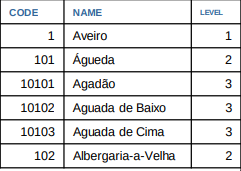
\includegraphics[width=0.4\linewidth]{figures/hierarchicalquery.png}
    \caption{Query result}
    \label{fig:hierarchicalquery}
\end{figure}

\newpage  
\subsubsection{Objects}

The main goal of an object is to deal with complex object. There're two ways that an object can be represented in a databases:

\begin{itemize}
    \item It can be \textbf{store as a table column}
    \item As the \textbf{row of a column}
\end{itemize}

The advantages of using objects are:
\begin{itemize}
    \item It \textbf{encapsulates} the data and thus can be \textbf{reused};
    \item We are able to store the OO programming structures without conversion. It eases the development. 
    \item Representation of part-of hierarchies. Hierarchies are important, since it might ease the representation of some structures and allow a better understandment. 
    \item It's more efficient, since fetch a group of objects in a a single access.
\end{itemize}

\subsubsubsection{Object types}  

Firstly, an object contains attributes and methods at the same time and is semantically richer than the convetional databases, but this can be also a disadvantage: it hides part of the structure (as it will be shown later) and the access should must be made through specific methods. Also, it's possible to have type inheritance. 

\subsubsubsection{Domain definition}   

A type can be seen as a domain (i.e a static infinite set where the column may pick values). 

\begin{lstlisting}

    create type address_t as object(
        street varchar2(30),
        zipcode varchar2(10),
        town varchar2(20),
        countryu varchar2(20)
    );

    create type position as object(
        position varchar2(20),
        start date,
        end date
    );
\end{lstlisting} 

\begin{tcolorbox} 
    The \texttt{varchar2} is different from \texttt{varchar}. The \texttt{varchar} sould not be used and is an internal type of oracle, while \texttt{varchar2} is an external variable and can be used by the user. More than that, \texttt{varchar2} does not distinguish between a \texttt{NULL} string and an empty string (i.e null = ''), however \texttt{varchar} makes this difference. 
\end{tcolorbox} 

\subsubsubsection{Objects as table columns} 

Types can be used as domains in table columns an in this case the objects are in the table columns.

\begin{lstlisting}
    create table members (
        ID number(10) primary key,
        name varchar2(20),
        address address_t,
        position position_t
    );
\end{lstlisting}

Let's see and example of how to add a row for the \texttt{members} table: 

\begin{lstlisting}

    insert into members(
        3658,
        'Besouro'
        address_t(
            "Rua de Soares dos Reis",
            "4400-163",
            "Vila Nova de Gaia",
            "Portugal"
        ),
        position_t(
            "President",
            "2010-01-01",
            "2012-12-31"
        )
    );
\end{lstlisting}

To perform \textbf{queries} and select an object, a cursor is necessary:

\begin{lstlisting}
    select name, m.address.street, position
    from members m where id=3658;
\end{lstlisting} 

\subsubsubsection{Object as table rows} 

\begin{lstlisting}
    create type department_t as object(
        acronym varchar2(5),
        designation varchar2(20),
        director number(10)
    );

    create deparments of deparment_t;
\end{lstlisting}

This is table was generated from type defined by the user and \textbf{contains objects}. This is not a normal table, since the object-row occupies the full row, while the object columns don't. The table \textbf{can be seen as a single column} of objects or multicolumn, like a relational table:

\begin{lstlisting}
    insert into departments values('CUL', 'Cultural', 3658); -- A multicolumn table
    insert into departments values(department_t('BIB', 'Biblioteca', 3658)); -- A single column
\end{lstlisting}

This is an example of the relation class=table approach. 

There're two ways that the values o the table can be retrieved. One of the ways of retrieving the information. 

\begin{lstlisting}
    select * from departments where director=3658;
\end{lstlisting} 

The result be something like this:

\begin{table}[h]
    \centering
    \begin{tabular}{|l|l|l|}
        \hline
        ACRONYM & DESIGNATION & DIRECTOR \\ \hline
        CUL     & Cultural    & 3658     \\ \hline
        BIB     & Biblioteca  & 3658     \\ \hline
    \end{tabular}
\end{table}

And the other way is:

\begin{lstlisting}
    select value(d) from departments d where director=3658;
\end{lstlisting}

In this result we have an object view:

\begin{table}[h]
    \centering
    \begin{tabular}{|l|}
    \hline
    VALUE(D) \\ \hline
    [DEPARTMENT\_T] \\ \hline
    [DEPARTMENT\_T] \\ \hline
    \end{tabular}
\end{table}

\subsubsubsection{Access object-row address}  

The object rows possess address, while objects in columns don't. 

\begin{lstlisting}
   select ref(d) from departments d; 
\end{lstlisting} 

The visualization, however, is automatically converted by SQL. In the result should be the same as performing a query with \texttt{value(d)}. This change may not affect the visualization, but might be useful programatically as we gonna see in the next. 

\subsubsubsection{references (REF)}

\textbf{What is the advantage of using references (REF)?}

The explain this question, let's first change the object column \texttt{address} in the \texttt{members} table to a reference to the class table \texttt{department\_t}.

\begin{lstlisting}  
    -- Remembering what the format of the member row.
    create table members (
        ID number(10) primary key,
        name varchar2(20),
        address address_t,
        position position_t
    );

    alter table members add (department ref department_t);
\end{lstlisting}

Now let's suppose we want to update department of some members:

\begin{lstlisting}
    update members set department = (select ref(d) from departments d where sigla='CUL') 
    where id=3658;
\end{lstlisting}

The advantage in this query is that we can have access to the table \texttt{departments} without performing a join.


 

    \end{document}  

% ---------------------
% Bibliography
% --------------------- 
% A folder bst/report.bib should be created 

\bibliographystyle{unsrt}
\bibliography{bst/report}  

